\documentclass[border=10pt]{standalone}
\usepackage{pgfplots}
\pgfplotsset{compat=1.17}
\begin{document}
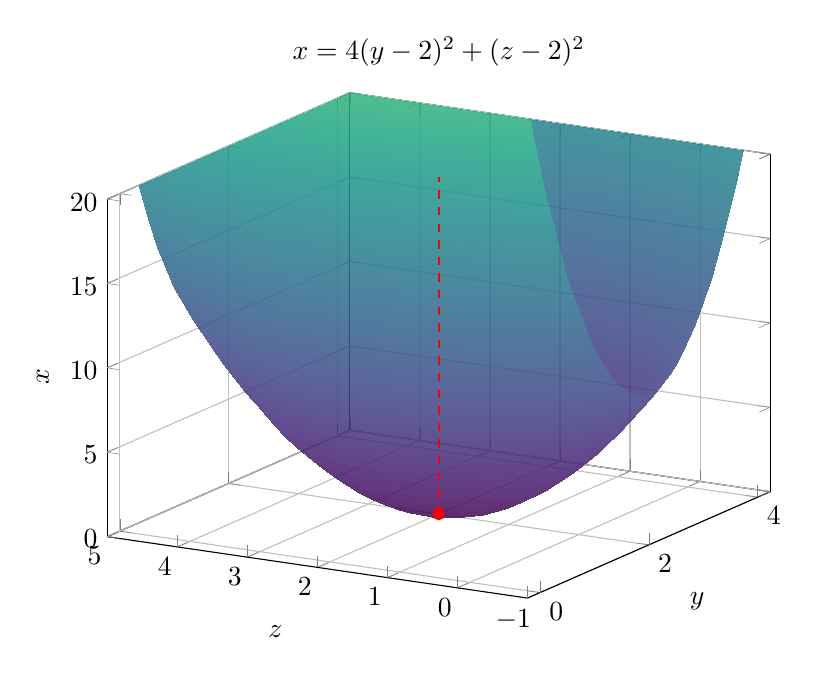
\begin{tikzpicture}
\begin{axis}[
    xlabel={$y$}, ylabel={$z$}, zlabel={$x$},
    title={$x=4(y-2)^2+(z-2)^2$},
    view={-60}{20},
    colormap/viridis,
    samples=40,
    domain=-1:5,
    y domain=-1:5,
    zmin=0, zmax=20,
    axis equal image=false,
    width=10cm, height=8cm,
    grid=both,
]
\addplot3[surf,shader=interp,opacity=0.85] {4*(x-2)^2+(y-2)^2};
\addplot3[red,mark=*,mark size=2pt] coordinates {(2,2,0)};
\addplot3[red,dashed,thick] coordinates {(2,2,0) (2,2,20)};
\end{axis}
\end{tikzpicture}
\end{document}
